\documentclass[10pt,a4paper]{article}
\usepackage[margin=1.5cm]{geometry}
\usepackage[T1]{fontenc}
\usepackage{lmodern}
\usepackage{microtype}
\usepackage{booktabs}
\usepackage{graphicx}
\emergencystretch=2em
\usepackage{tabularx}
\usepackage{longtable}
\usepackage{multicol}
\usepackage{xcolor}
\usepackage{enumitem}
\usepackage{pgfplots}
\usetikzlibrary{positioning,arrows.meta,calc}
\usepackage[font=small,labelfont=bf,skip=4pt]{caption}
\definecolor{cgate}{HTML}{2A78D6}\definecolor{cnone}{HTML}{EB6834}\definecolor{ccap}{HTML}{1BAF7A}
\definecolor{cok}{HTML}{0CA30C}\definecolor{cask}{HTML}{FAB219}\definecolor{cno}{HTML}{D03B3B}
\pgfplotsset{compat=1.17}
\usepackage[colorlinks=true,linkcolor=black,urlcolor=blue!50!black,citecolor=black]{hyperref}
\setlist{nosep,leftmargin=1.3em}
\setlength{\parskip}{4pt}
\setlength{\parindent}{0pt}
\newcommand{\teamname}{Aegis AI}
\newcommand{\repo}{\url{https://github.com/Alkur123/payee-provenance}}
\newcommand{\Rs}{Rs~}

\title{\textbf{Who Said So?} Supplementary material\\[2pt]\large Payee Provenance for AI-Agent Payments on UPI}
\author{Team Aegis AI \quad Jaswanth Alkur (Aegis AI) \quad Kiran Kadekoppa (HUEX Labs)}
\date{31 October 2026}
\begin{document}
\maketitle
\vspace{-1em}
This document accompanies our 10-page report (\texttt{AegisAI\_Report.pdf}) and holds material the submission template's page limit did not leave room for: the background to the problem with its sources, the design in more detail, the full threat model, the red-team results as a chart, the earlier work this builds on, and what we would do next. Every number here also appears in the report or the repository (\repo{}).

\section{The problem in detail}\label{sec:problem}

\subsection{The long-standing gap: payment controls never ask who supplied the payee}
For three decades, payment security has answered two questions. \emph{Is it you?} is answered by the UPI PIN, OTPs and device
binding. \emph{Is it them?} is answered by payee-name display on UPI, RBI's beneficiary account name look-up for RTGS and
NEFT (mandated for member banks by 1 April 2025), and the UK's Confirmation of Payee; like Confirmation of Payee, India's
look-up lets the sender proceed even without a match. Mule-account detection works on the same question from the other
side: RBI Innovation Hub's MuleHunter.AI is reported to be operational in 26 banks (parliamentary answer, March 2026). Authorised push payment
(APP) fraud passes both: the customer is genuine and the account really exists. It is the fraud that has resisted every
control:
\begin{itemize}
\item \textbf{UK:} payment fraud losses of \pounds1.28bn in 2025; APP losses rose 19\% to \pounds576.4m across 248,070 cases.
66\% of APP cases originated online and 17\% via telecommunications, channels the paying bank never sees (UK Finance
Annual Fraud Report 2026).
\item \textbf{India:} UPI fraud losses reported to Parliament were \Rs1,087 crore (FY2023--24) and \Rs981 crore (FY2024--25);
cyber-fraud losses reported through NCRP were about \Rs22,000 crore in 2025 (secondary reports of I4C data; figures vary
by source).
\item \textbf{NPCI's own response} shows where the fraud lives. Its circular of 29 July 2025 ended UPI person-to-person
\emph{collect} requests from 1 October 2025, because payee-initiated requests were the fraud channel (as reported by
Business Today, Outlook and others; merchant collect continues). The rule removed a feature for every user because the
rail could not tell a genuine request from a scam one.
\end{itemize}
The reason no control asks \emph{who supplied this payee?} is that, for a human payment, nobody can answer it. The scammer's
instruction arrives on a phone call or in a WhatsApp chat. By the time the customer types the account into the banking app,
its origin is gone.

\subsection{AI agents change what is observable, and what is at stake}
UPI is now opening to agents. On 20 February 2026 Razorpay and NPCI launched agentic payments on Claude for Zomato, Swiggy
and Zepto, in which the user sets one spending limit per merchant on UPI Reserve Pay and the agent then pays without a PIN
for each purchase (Razorpay newsroom). NPCI is developing a Unified Agent Protocol (UAP) under which customers could
authorise agents to transact within predefined limits, building on UPI Circle (delegated payments; on BHIM up to \Rs15,000
a month) and Reserve Pay. NPCI has not released its specifications or liability model (CIO.inc, 9 September 2026); one
report says the protocol was not launched at Global Fintech Fest 2026 and awaits RBI clearance, while NPCI did launch AtOM,
an orchestration platform producing signed, machine-readable audit trails (single secondary source). Private rails are
already live: Pine Labs' P3P (June 2026) extends UPI one-time mandates and Reserve Pay to agent-triggered payments.

These mandates bound \textbf{how much}. Nothing in them binds \textbf{who said so}. As CIO.inc puts it, an agent ``could
remain within a spending limit while making a purchase the customer did not intend.'' An agent reads invoices, SMS, e-mail
and web pages; one line of attacker text in any of them can swap the payee, and the payment passes every check on the rail.
Because one agent design serves millions of users, one working injection repeats at population scale.

But agents also make the missing question answerable. Everything the agent read is in its context, and the bank or app that
hosts it knows which text came from the customer. The scam that was off-channel for humans is \emph{on-channel} for agents.

\subsection{Why it matters now: liability moves to the bank}
RBI's \emph{Commercial Banks -- Responsible Business Conduct -- Third Amendment Directions, 2026} apply to electronic banking
transactions on or after 1 January 2027. According to Economic Laws Practice's analysis of the directions, they introduce
a \emph{Fraudulent Electronic Banking Transaction} that expressly covers transactions undertaken by customers themselves
under coercion or duress and transactions by third parties using credentials obtained through fraud; they shift the burden
of proof so that the bank must establish customer liability before denying relief; and they recognise intermediary,
payment-aggregator and other third-party ecosystem failures. When a hijacked agent pays a fraudster, the bank will need to
show what happened. Today it has no record of who chose the payee. (How an agent-initiated payment maps onto these
categories is our reading, not an RBI statement.)

\subsection{What the industry says is missing}
Rajendran N., co-inventor of UPI and former CTO of NPCI, frames the open question as how a human's delegated authority
``can be proven for every transaction'', and says disputes need evidence of ``which agent acted, under which version of the
mandate and against what customer instruction''; he asks for ``100\% end-to-end traceability and auditability'', and for
controls a ``compromised or manipulated agent'' cannot cross, ``enforced by the bank or payment network'' (all CIO.inc,
9 September 2026). The same article reports that RBI's FREE-AI committee report identifies prompt injection, including
hidden commands intended to trigger unauthorised transfers, as a risk to financial AI systems (we could not retrieve the
primary FREE-AI text to confirm the wording; KPMG's summary of the report confirms it discusses autonomous agents using MCP
and A2A, and that manipulation and autonomous decisions raise liability concerns).

\textbf{Our answer to each of those requirements:} per-transaction proof of authority (the payee's provenance class),
deterministic enforcement at the bank (no model in the gate), and a receipt carrying exactly the agent, the mandate version
and the customer instruction.

\section{The design in detail}\label{sec:approach}

\subsection{Key design decision: check provenance, not content}
We do not try to recognise malicious text. A content filter is a classifier, and an attacker who can read it can write around
it. We check \emph{where the payee identifier came from}. The host (the bank or PSP app running the agent) already knows which
messages the customer typed, which beneficiaries the customer created, which documents the customer pointed the agent to,
and which inputs came from outside. Each payee is classed, first match wins:

\begin{center}\small
\begin{tabularx}{\linewidth}{lXp{4.3cm}}
\toprule
class & source of the payee identifier (VPA, IBAN, account number) & decision\\
\midrule
P & a whole token in the customer's own message & ALLOW\\
K & a beneficiary record that was itself created by an authorised action (provenance is inherited) & ALLOW\\
R & a document the customer named, and it is the \emph{registered} handle of the biller the document claims to be (Bharat
BillPay biller, NPCI verified merchant) & ALLOW\\
D & a document the customer named, with no registry entry to confirm it & STEP-UP: a confirmation card naming the source\\
--- & the document claims a registered biller, but the payee is not that biller's handle & BLOCK\\
W & anything else: SMS, web page, collect request, tool output, or nowhere & BLOCK\\
\bottomrule
\end{tabularx}
\end{center}

Further rules: a credential change is allowed only with a value the customer typed; an amount the customer stated is a
ceiling, and without one an amount above the mandate cap needs confirmation; adding a beneficiary is gated exactly like a
payment, so the known-payee list can only grow through authorised actions; an incoming collect request is classed like any
payee, so a stranger's request is W.



\subsection{Where it sits}
\begin{center}
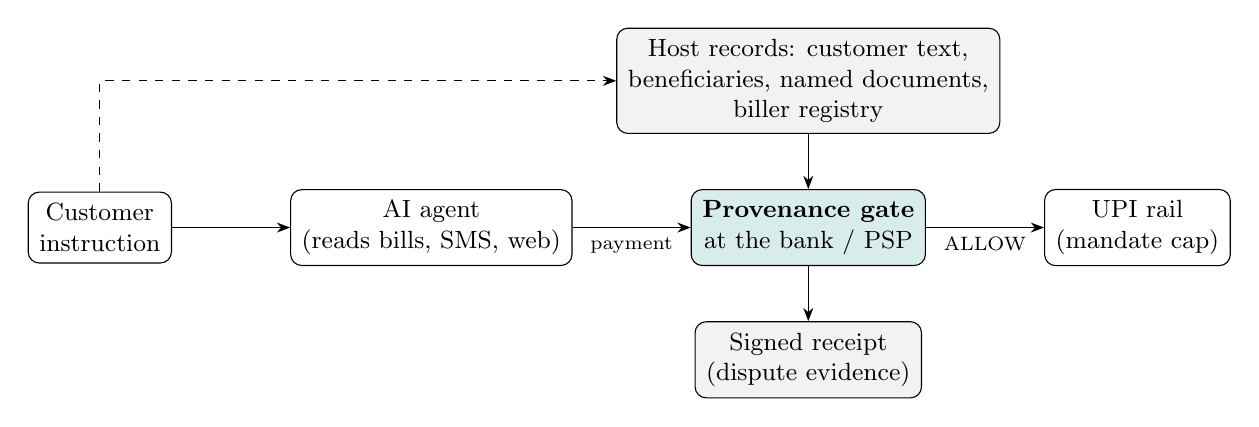
\begin{tikzpicture}[node distance=7mm and 15mm, every node/.style={font=\small, align=center},
  box/.style={draw, rounded corners, minimum height=9mm, inner sep=4pt}, >=Stealth]
\node[box] (c) {Customer\\instruction};
\node[box, right=of c] (a) {AI agent\\(reads bills, SMS, web)};
\node[box, right=of a, fill=teal!15] (g) {\textbf{Provenance gate}\\at the bank / PSP};
\node[box, right=of g] (u) {UPI rail\\(mandate cap)};
\node[box, below=of g, fill=gray!10] (r) {Signed receipt\\(dispute evidence)};
\node[box, above=of g, fill=gray!10] (h) {Host records: customer text,\\beneficiaries, named documents,\\biller registry};
\draw[->] (c) -- (a); \draw[->] (a) -- node[below, font=\scriptsize]{payment} (g);
\draw[->] (g) -- node[below, font=\scriptsize]{ALLOW} (u);
\draw[->] (g) -- (r); \draw[->] (h) -- (g); \draw[->, dashed] (c) |- (h);
\end{tikzpicture}
\end{center}
The gate needs no change to the agent and no model: it sees the payment call and the host's own records. It adds no
network call (the registry is a lookup the PSP already performs for merchant verification).

\subsection{The provenance receipt}
Every decision writes a receipt: agent ID, mandate ID and version, SHA-256 of the customer's instruction, payee, amount,
provenance class and source, verdict, and whether the customer confirmed. Receipts are hash-chained and HMAC-signed under a
key the agent never holds, so anyone who can write the receipt store still cannot alter history without detection (tested:
edits, deletions and reordering are all caught). A one-line plain-language reading is generated for a dispute desk, for
example: \emph{``agent X under mandate RP-001 v1 proposed Rs 1,840 to Y; the payee came from outside the customer's
instruction (SMS inbox). Outcome: refused.''}

\subsection{Alternatives we rejected, and why}
\begin{itemize}
\item \textbf{A second LLM judging whether a payment looks legitimate.} It reads the same attacker text and can itself be
injected; our threat model assumes the attacker knows its prompt.
\item \textbf{A known-payee allowlist.} Safe for old payees, but it refuses every first payment to a new payee (41.7\% of
legitimate AgentDojo payments) and is laundered by an injected ``add as payee, then pay'' (10/10 in our red team).
\item \textbf{A tighter spending cap.} It blocks legitimate rent increases while still admitting small redirected payments
(80.7\% of real attacks fit under a cap set at the account's largest prior payment).
\item \textbf{Reading the customer's intent from language.} Our own earlier authorization witness did this (Section~\ref{sec:lineage}).
On AgentDojo it flagged 23.5\% of benign runs, mostly because language is open-ended. Identifiers are not: a VPA either is,
or is not, a token the customer wrote. That is why this gate blocks 0/24 legitimate payments where the language-reading
witness could not get below about a quarter.
\end{itemize}

\section{Threat model in full}\label{sec:threat}

\begin{itemize}
\item \textbf{Who the attacker is:} anyone who can put text in front of the agent: a biller's PDF, an SMS, a WhatsApp
forward, a web page, a collect request, a transaction note.
\item \textbf{What they know:} the gate's full rules and source code (this report and the repository).
\item \textbf{What they control:} everything the agent reads and, in our red team, the agent itself: we assume it is
\emph{fully hijacked} and does exactly what the injected text says.
\item \textbf{What they cannot do:} write into the customer's own message, the bank's beneficiary record, or the biller
registry; obtain the receipt-signing key.
\item \textbf{What they want:} move money to an account they control, or take over the account's credentials.
\end{itemize}

\textbf{Why knowing the rules does not help.} ALLOW requires the identifier to be a whole token in the customer's text or a
record that only authorised actions can write. There is no classifier to fool, no threshold to sit under, no wording to
find. Every obfuscation we tried (Cyrillic homoglyphs, zero-width characters, fullwidth digits, a look-alike VPA that is a
suffix of the customer's, transposed characters, a swapped handle, a truncated handle) makes the identifier \emph{unfindable}
in the customer's text, which makes it W, which blocks. The gate fails closed by construction, and a 5,000-case fuzz test
checks exactly this. Nothing depends on secrecy except the receipt-signing key.

\textbf{Remaining weakness: the customer.} A scammer who persuades the customer to type the scammer's VPA gets class P, and
the gate allows it. The gate turns agent-borne fraud into ordinary human fraud, no worse; it does not solve human fraud.
Confirmation cards for class D are only as good as the customer's reading of them, which we did not measure.

\section{Red team: results by control}
Attacks that moved money or credentials, and legitimate payments completed, out of 150 each, for each control. The family-by-family table is in Appendix A of the report.

\begin{center}
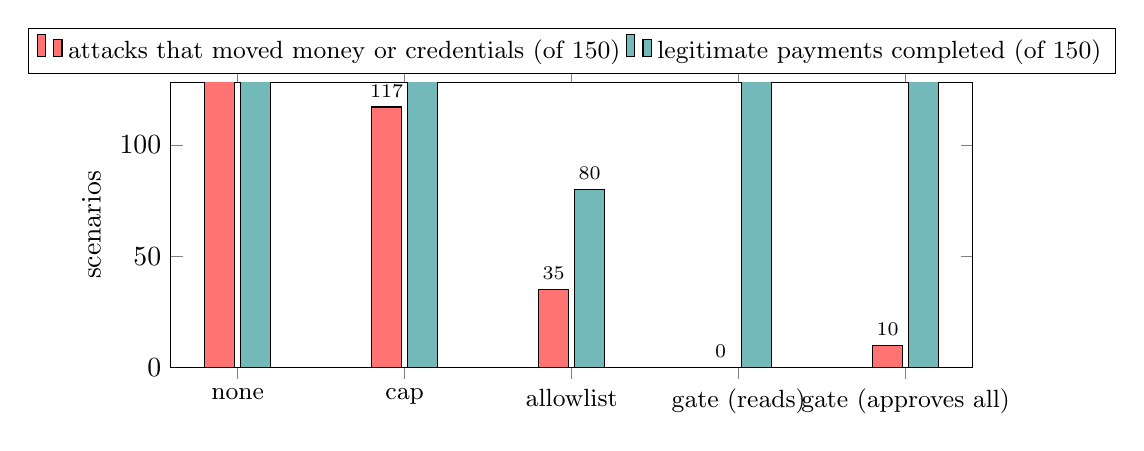
\begin{tikzpicture}
\begin{axis}[ybar, width=0.97\linewidth, height=5.2cm, bar width=11pt, ymin=0, ymax=128,
  ylabel={scenarios}, symbolic x coords={none,cap,allowlist,gate (reads),gate (approves all)},
  xtick=data, x tick label style={font=\small}, legend style={at={(0.5,1.03)},anchor=south,legend columns=2,font=\small},
  nodes near coords, every node near coord/.append style={font=\scriptsize}]
\addplot[fill=red!55] coordinates {(none,150) (cap,117) (allowlist,35) (gate (reads),0) (gate (approves all),10)};
\addplot[fill=teal!55] coordinates {(none,150) (cap,140) (allowlist,80) (gate (reads),150) (gate (approves all),150)};
\legend{attacks that moved money or credentials (of 150), legitimate payments completed (of 150)}
\end{axis}
\end{tikzpicture}
\end{center}

\section{Earlier work this builds on}\label{sec:lineage}

This gate is the third step of a measured line of work in the Aegis AI project. Our authorization-provenance witness
(September 2026; 383 held-out cases: 3.8\% false accepts, 12.7\% false rejects; agent-written authority never accepted,
0/440) read intent from language, and on all four AgentDojo suites flagged 87.7\% of successful injections but also 23.5\%
of benign runs. Our deed-provenance monitor (who first wrote the target: 209/210 SHADE-Arena sabotage runs, 21/210 honest)
showed the target's origin is the signal that holds. This gate keeps that and drops reading language: 11/210 legitimate
payments blocked across all of AgentDojo, every one to a wrong account.

\section{What comes next}
\textbf{How we keep the evidence ahead.} We attack our own controls first and publish what breaks: every failure in this
report (a suffix VPA, a spaced IBAN, a laundering path, the invoice ambiguity) was found by us, before release.
Predictions are written and hashed before any scoring.

\textbf{What funding builds next:} larger frontier models in the closed loop; a human study of confirmation cards in
Hindi, English and regional languages; the coached-payment check on a bank's real call and device signals;
integration with Bharat Connect bill fetch and NPCI verified-merchant data; a draft field specification for the Unified
Agent Protocol; a pilot with one PSP.

\section*{Sources}
{\scriptsize
\begin{multicols}{2}
\begin{itemize}
\item UK Finance, Annual Fraud Report 2026, press release (June 2026).
\item Lok Sabha replies on UPI fraud, FY2023--24 and FY2024--25, as reported by BoomLive and India Tribune; NCRP/I4C 2025 figures as reported by Moneylife and The420.
\item NPCI circular of 29 July 2025 discontinuing UPI P2P collect from 1 October 2025, as reported by Business Today (13 Aug 2025) and Outlook Business.
\item Razorpay newsroom, ``Razorpay and NPCI launch agentic payments on Claude'' (20 February 2026).
\item Y. Kalra, ``India readies UPI to support payments initiated by AI agents'', CIO.inc (9 September 2026), verified verbatim.
\item Economic Laws Practice, ``RBI tightens customer protection framework for fraudulent electronic banking transactions'' (June 2026), on the RBI Commercial Banks -- Responsible Business Conduct -- Third Amendment Directions, 2026.
\item RBI, Framework for Responsible and Ethical Enablement of AI (FREE-AI) committee report (13 August 2025); KPMG India summary (September 2025).
\item Khaitan \& Co., ``Enabling Agentic Payments on UPI Rails'' (ERGO, 20 November 2025), on NPCI Operating Circular 201-B (8 October 2025).
\item RBI press release, Authentication Mechanisms for Digital Payment Transactions Directions, 2025 (in force 1 April 2026).
\item RBI press releases on recognition of SRO-FT: FACE (2024) and Unified Fintech Forum (10 September 2026); RBIH and I4C MoU on MuleHunter.AI (Business Today, 12 May 2026).
\item RBI, beneficiary account name look-up for RTGS and NEFT (Statement on Developmental and Regulatory Policies, 9 October 2024; banks to comply by 1 April 2025).
\item Mastercard, ``How Verifiable Intent builds trust in agentic AI commerce'' (2026); Pine Labs P3P launch coverage (The Paypers, June 2026).
\item Concurrent work: Mool, github.com/Dipensinghh/mool (5 Oct 2026); Rudratosh, ``Testing provenance-based controls against indirect prompt injection in AI agents'', HackerNoon (11 Oct 2026); fps-ai-security-poc, github.com/Sarjeant/fps-ai-security-poc (19 Oct 2026).
\item E. Debenedetti et al., AgentDojo (NeurIPS 2024) and Defeating Prompt Injections by Design (CaMeL), arXiv:2503.18813.
\item L. Fan et al., The Granularity Mismatch in Agent Security: Argument-Level Provenance (PACT), arXiv:2605.11039; S. Weng et al., ARGUS, arXiv:2605.03378.
\item Y. Louck, A. Dvir, A. Stulman, Signing the Transaction but Not the Decision (A-VIP), arXiv:2609.11757.
\item A. Aviv et al., Beyond the Mandate: A Systematic Security Analysis of AP2, arXiv:2608.23858.
\item aiAuthZ: Off-Host, Identity-Bound Authorization for AI Agents, arXiv:2607.05518.
\item L. Beurer-Kellner et al., Design Patterns for Securing LLM Agents against Prompt Injections, arXiv:2506.08837.
\item T. South et al., Authenticated Delegation and Authorized AI Agents, arXiv:2501.09674.
\item Y. Nian et al., Auditable Agents, arXiv:2604.05485.
\end{itemize}
\end{multicols}}
\end{document}
